\documentclass[main.tex]{subfiles}
 
\begin{document}
In this final chapter, we 

\section{SciGRID data}
The SciGRID dataset needs to be translated into the language of our model. It contains more information than we need, and it is not yet in the desired format. 

\subsection{Structure}
\emph{(A more detailed analysis of dataset properties is available on the GitHub repository.)}

Before any processing, we find that the SciGRID network (obtained from \texttt{PyPSA} example code, the exact dataset used by \cite{Nesti2018emergentfailures}) contains 585 buses, 1423 generators (of all sources) and 489 loads. It also contains 38 storage units (all are pumped hydroelectric), but these were excluded from our analysis.\footnote{More specifically, they were used in solving the OPF problem, but their initial charge was set to zero.} There are 852 transmission lines in the dataset, at possible voltage levels $220 \, \si{\kilo\volt}$ and $380 \, \si{\kilo\volt}$, and there are 96 transformers (between these two voltages). Transmission lines have per-kilometre estimates for admittance, from which the total admittance can be deduced.

\subsubsection{Voltages}
In our model, we \emph{normalise} the grid voltage. To do so, we multiply all line admittances by the \emph{square} of their operating voltages, after which all voltages can be assumed to be $1$, and a unit of current is proportional to a unit of transmitted power. Of the 585 buses, 192 are part of one of the 96 \emph{voltage pairs}: these are two buses at the same location, with the same name (except for the voltage suffix), connected via a transformer. By merging these pairs, we find 489 geographically unique buses, at normalised voltage. From now on, we will refer to these (possibly merged) buses as the buses of the network: $n=489$, $\mathcal{N} = \range{489}$.

\subsubsection{Loads}
There is exactly 1 load connected to each bus. In reality, there are of course thousands of loads connected to a bus, but the load in the dataset is the \emph{aggregated} load at that bus. We have hourly time series (\ie amount of $\si{\mega\watt}$ being consumed) for each node in the year 2011, which only includes active power consumption.

\subsubsection{Generators}
Generators are connected to the geographically closest bus, and there is at most one generator per bus of each type.\footnote{In order of installed capacity: \emph{Wind Onshore} ($37\,\si{\giga\watt}$), \emph{Solar} ($37\,\si{\giga\watt}$), \emph{Hard Coal} ($25\,\si{\giga\watt}$), \emph{Gas} ($24\,\si{\giga\watt}$), \emph{Brown Coal} ($21\,\si{\giga\watt}$), \emph{Nuclear} ($12\,\si{\giga\watt}$), \emph{Run of River} ($4\,\si{\giga\watt}$), \emph{Other} ($3\,\si{\giga\watt}$), \emph{Wind Offshore} ($3\,\si{\giga\watt}$), \emph{Oil} ($2.7\,\si{\giga\watt}$), \emph{Waste} ($1.6\,\si{\giga\watt}$), \emph{Storage Hydro} ($1.4\,\si{\giga\watt}$), \emph{Multiple} ($0.15\,\si{\giga\watt}$) and \emph{Geothermal} ($32\,\si{\mega\watt}$).} This means that generation is \emph{aggregated}: multiple generators of the same type are combined into one. There are 489 solar generators, 488 onshore wind generators and 5 offshore wind generators. Offshore wind generators are connected to buses at the north coast of Germany. This means that every bus houses stochastic generation. Their geographic distribution is shown in Figure~\ref{fig:solarwind}.

\subsubsection{Lines}
Line voltages and admittances are normalised as described above. For each line, we have the names of the two original buses that it connects, which can easily be converted to the new bus collection.

During the study of cascading failures, we found that the network contains \emph{parallel lines}: lines that connect the same pairs of buses. In some cases, there are up to four different lines that are all parallel. When examining these cases on OpenStreetMap, we find that there are indeed parallel lines in the physical network. This is reflected by the \emph{lengths} of parallel lines, as given by SciGRID: these are not the great-circle distances between buses, but rather the distance measured along the line (which makes some turns and bends).

Because our model only holds for \emph{digraphs}, which cannot have parallel lines, we \emph{combine} parallel lines, by summing their (voltage normalised) admittances, and summing their thresholds.\footnote{The results regarding the kernel of $\FRT$, and the Optimised method for analysis cascading failures, break down without this property.} \cite{Nesti2018emergentfailures} do not mention this anomaly, and use the original set of lines. For comparison, we computed some results for both versions of the network, and found the results to be somewhat similar, in general. Because we did not consider the case of parallel lines in our model, combining parallel lines in the dataset seems like the \emph{correct} choice.

Of the 852 original lines, there are 705 unique links between original buses before normalising voltages, and there are 695 unique links between buses. There are never two parallel lines with opposite orientation. These 695 lines were used in our model, and will be referred to as simply the \emph{lines} of the network: $m = 695$.

\subsection{State}
Our dataset contains hourly values for load and stochastic (wind and solar) generation for the year 2011. Deterministic generation is estimated using the OPF algorithm, as implemented by \texttt{PyPSA} \citep{PyPSA}, a Python package designed for this purpose. Following common practice, we first multiply all line thresholds by a \define{contingency factor}: $0.70$. This forces the optimisation process to leave a safety margin at every line, and also accounts for the error of using the DC approximation. Figure~\ref{fig:nominalflowandinjection} shows the resulting injection at 1 January 2011 at 11:00. Line currents can then be computed using the LPF.

\begin{figure}[ht]
    \centering
    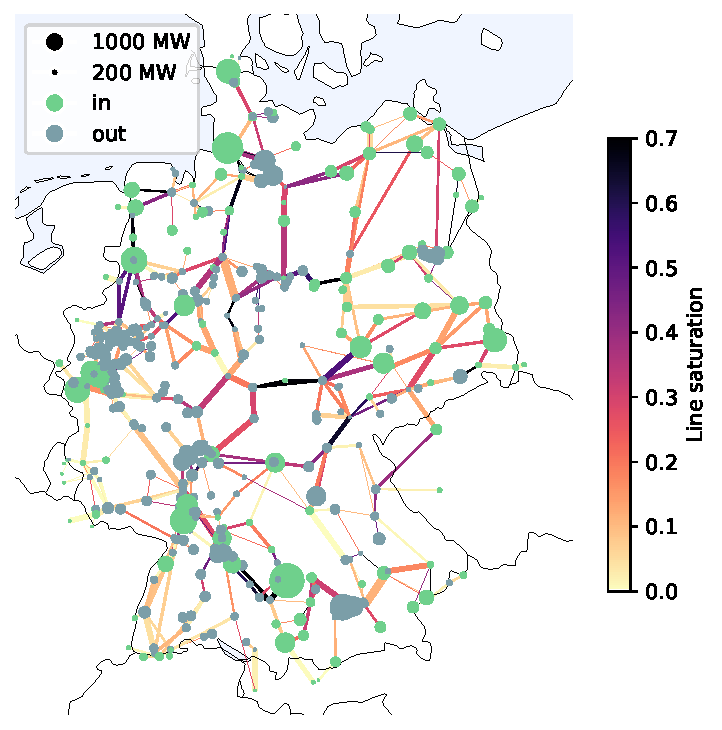
\includegraphics[width=.6\textwidth]{img/nominal_flow_and_injection.pdf}
    \caption{
    \label{fig:nominalflowandinjection}Nominal line flow during 11:00-12:00, as fraction of line capacity. Node size represents net power injection. When generation exceeds load, the injection is positive (green), otherwise negative (greyish blue). \emph{Compare with Figure 1a of \cite{Nesti2018emergentfailures}.}}
\end{figure}

\section{Bus covariance}

\begin{figure}[ht]
    \centering
    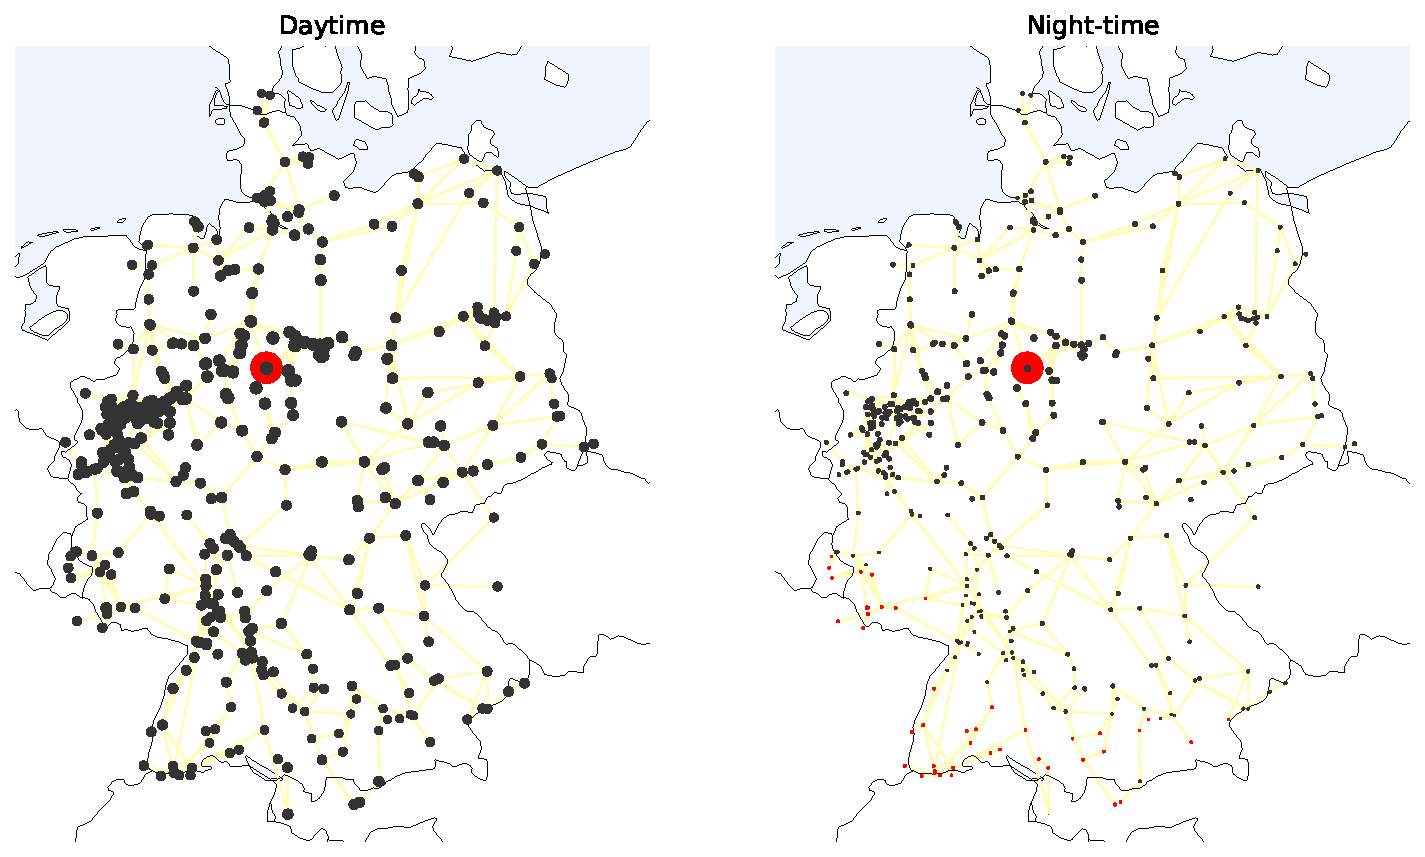
\includegraphics[width=\textwidth]{img/bus_correlation_123_fullcov_day_and_night.pdf}
    \caption{
    \label{fig:buscov}Covariance of all buses, relative to the circled bus. Normalised using installed renewable capacity.}
\end{figure}


\begin{table}[]
    \centering
    \begin{tabular}{c|ccrr|ccrr}
\toprule
\multicolumn{1}{c}{} & \multicolumn{4}{c}{\textsc{Solar}} & \multicolumn{4}{c}{\textsc{Wind}} \\
\midrule
\multicolumn{1}{c}{} & 
\multicolumn{1}{c}{\textit{default}} & \multicolumn{1}{c}{\textit{modified}} & 
\multicolumn{1}{c}{1\%} & \multicolumn{1}{c}{2\%} & 
\multicolumn{1}{c}{\textit{default}} & \multicolumn{1}{c}{\textit{modified}} & 
\multicolumn{1}{c}{1\%} & \multicolumn{1}{c}{2\%} \\
\midrule
Jan & \texttt{385} & \texttt{\textbf{484}} & \texttt{\textbf{5}} & \texttt{\textbf{0}} & \texttt{\textbf{488}} & \texttt{488} & \texttt{\textbf{0}} & \texttt{\textbf{0}} \\
Feb & \texttt{364} & \texttt{\textbf{485}} & \texttt{\textbf{4}} & \texttt{\textbf{0}} & \texttt{\textbf{487}} & \texttt{487} & \texttt{\textbf{0}} & \texttt{\textbf{1}} \\
Mar & \texttt{334} & \texttt{\textbf{475}} & \texttt{\textbf{14}} & \texttt{\textbf{0}} & \texttt{\textbf{487}} & \texttt{487} & \texttt{\textbf{1}} & \texttt{\textbf{0}} \\
Apr & \texttt{211} & \texttt{\textbf{477}} & \texttt{\textbf{11}} & \texttt{\textbf{1}} & \texttt{\textbf{488}} & \texttt{488} & \texttt{\textbf{0}} & \texttt{\textbf{0}} \\
May & \texttt{189} & \texttt{\textbf{473}} & \texttt{\textbf{16}} & \texttt{\textbf{0}} & \texttt{\textbf{467}} & \texttt{467} & \texttt{\textbf{21}} & \texttt{\textbf{0}} \\
Jun & \texttt{255} & \texttt{\textbf{481}} & \texttt{\textbf{8}} & \texttt{\textbf{0}} & \texttt{\textbf{480}} & \texttt{480} & \texttt{\textbf{8}} & \texttt{\textbf{0}} \\
Jul & \texttt{292} & \texttt{\textbf{485}} & \texttt{\textbf{4}} & \texttt{\textbf{0}} & \texttt{\textbf{488}} & \texttt{488} & \texttt{\textbf{0}} & \texttt{\textbf{0}} \\
Aug & \texttt{179} & \texttt{\textbf{478}} & \texttt{\textbf{10}} & \texttt{\textbf{1}} & \texttt{\textbf{488}} & \texttt{488} & \texttt{\textbf{0}} & \texttt{\textbf{0}} \\
Sep & \texttt{259} & \texttt{\textbf{472}} & \texttt{\textbf{16}} & \texttt{\textbf{1}} & \texttt{\textbf{487}} & \texttt{487} & \texttt{\textbf{1}} & \texttt{\textbf{0}} \\
Oct & \texttt{263} & \texttt{\textbf{480}} & \texttt{\textbf{9}} & \texttt{\textbf{0}} & \texttt{\textbf{488}} & \texttt{488} & \texttt{\textbf{0}} & \texttt{\textbf{0}} \\
Nov & \texttt{290} & \texttt{\textbf{472}} & \texttt{\textbf{17}} & \texttt{\textbf{0}} & \texttt{\textbf{486}} & \texttt{486} & \texttt{\textbf{2}} & \texttt{\textbf{0}} \\
Dec & \texttt{317} & \texttt{\textbf{482}} & \texttt{\textbf{7}} & \texttt{\textbf{0}} & \texttt{\textbf{486}} & \texttt{486} & \texttt{\textbf{2}} & \texttt{\textbf{0}} \\
\bottomrule
    \end{tabular}%TODO: modified wind bold?
    \caption{Number of buses (out of 489 solar, 488 wind) for which the ARMA model could be fitted using either the \emph{default} implementation of \texttt{arima} in \texttt{R}, or the \emph{modified} version (described in \ref{arimamod}).
    \newline
    When even the modified method yielded no results, uniform noise was added to the series before fitting. Noise magnitude was set to 1\% of generation capacity, or 2\% when needed.
    \newline
    Figures in \textbf{bold} indicate which results are used.
    %All nodes now have usable results.
    }
    \label{tab:arimafitstats}
\end{table}

\section{Line covariance}

By incorporating bus covariances in our model (which result from correlated weather), we hope to find new structure in the line covariances. 
To assess the effect of estimating bus covariances, we compare three possible bus covariance matrices:
\begin{enumerate}
	\item \emph{The identity matrix}: all bus injections are independently Gaussian distributed with the same variance. (They are almost IID, but their means differ.)
	\item \emph{The diagonal of estimated variances}: all bus injections are independently Gaussian distributed, but their variances and means differ.
	\item \emph{The estimated covariances}: the vector of bus injections is (multivariate) Gaussian distributed. All bus injections are, in general, dependent on each other, and their variances and means differ.
\end{enumerate}

It is well known that local changes to the grid structure have long-range effects. For example, \cite{Witthaut2013} showed that \emph{adding} a new line to a heavily congested, but stable network can cause the failure of another line, possibly far away from the added line.\footnote{The counter-intuitive fact that adding a line, or increasing the impedance of existing lines, can make a network \emph{more} congested, is known as \define{Braess' Paradox}. Similarly, some line failures can be \emph{prevented} by switching off other lines in the network. See Figure~\ref{fig:braess} for a minimal example.} This is reflected in our model by the fact that line currents have non-zero covariance, even when bus injections are independently distributed. (In this case, $\mat{\Sigma}_{\mat{f}} = \mat{F}\mat{I}\mat{F}^* = \mat{F}\mat{F}^*$, which is generally not a diagonal matrix.) Figure~\ref{fig:linecov1} and Figure~\ref{fig:linecov2} show the covariances of all lines, relative to a chosen line. We see that covariance is generally high for lines that are close, but there are some clear exceptions. There seems to be a general trend that lines are highly (positively or negatively) correlated when they are close, and \emph{oriented in the same direction} (\eg East-West) as the chosen line.



\begin{figure}
\centering
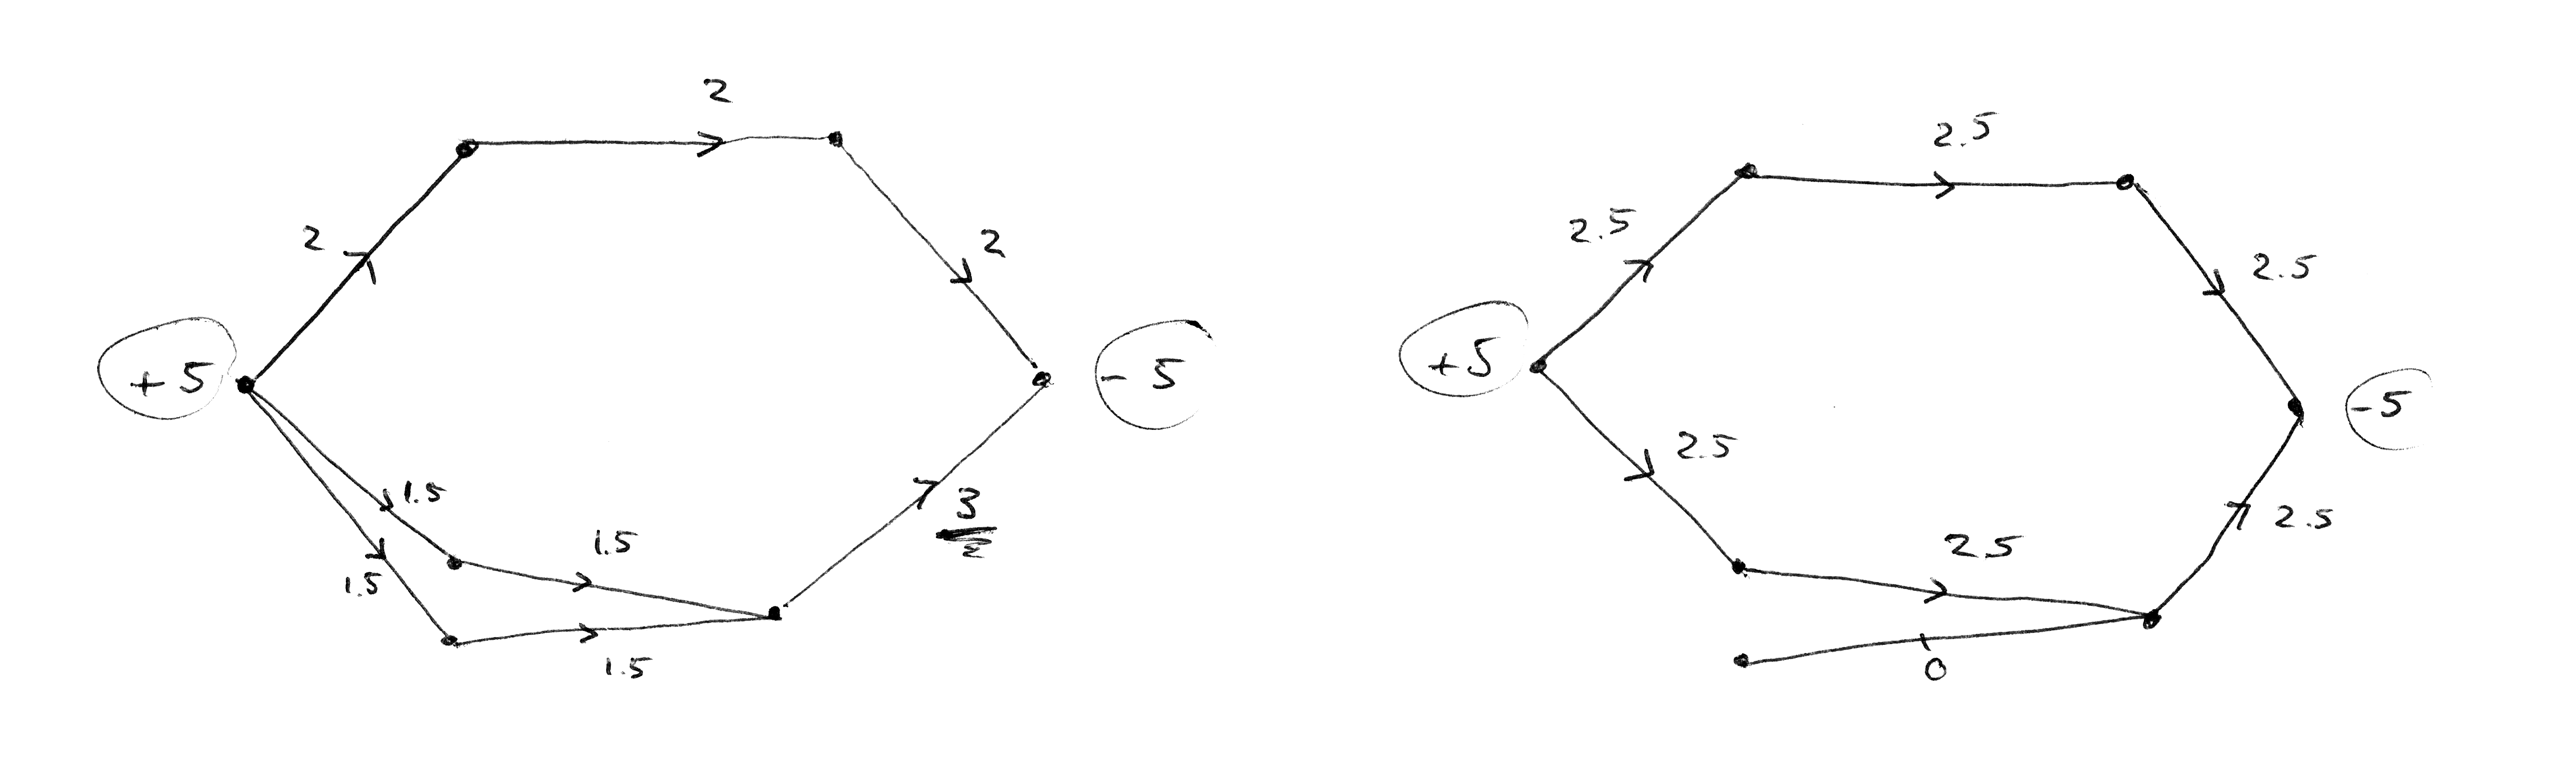
\includegraphics[width=\textwidth]{img/braesstekening.png}
\caption{\label{fig:braess} PLACEHOLDER: An example of Braess' Paradox. A network transporting $5$ units of power from left to right; all lines have the same admittance, and threshold $3$. On the left, one line (lower right) is overloaded. When this line fails, all power will travel through the upper branch, causing it to overload as well, leaving the network disconnected. If instead, the \emph{lower left} line is switched off, the flow of power will be more evenly distributed, and no line will overload. Of course, this example also illustrates how adding a line could lead to overloads.}
\end{figure}

\begin{figure}[ht]
\begin{subfigure}{\textwidth}
    \centering
    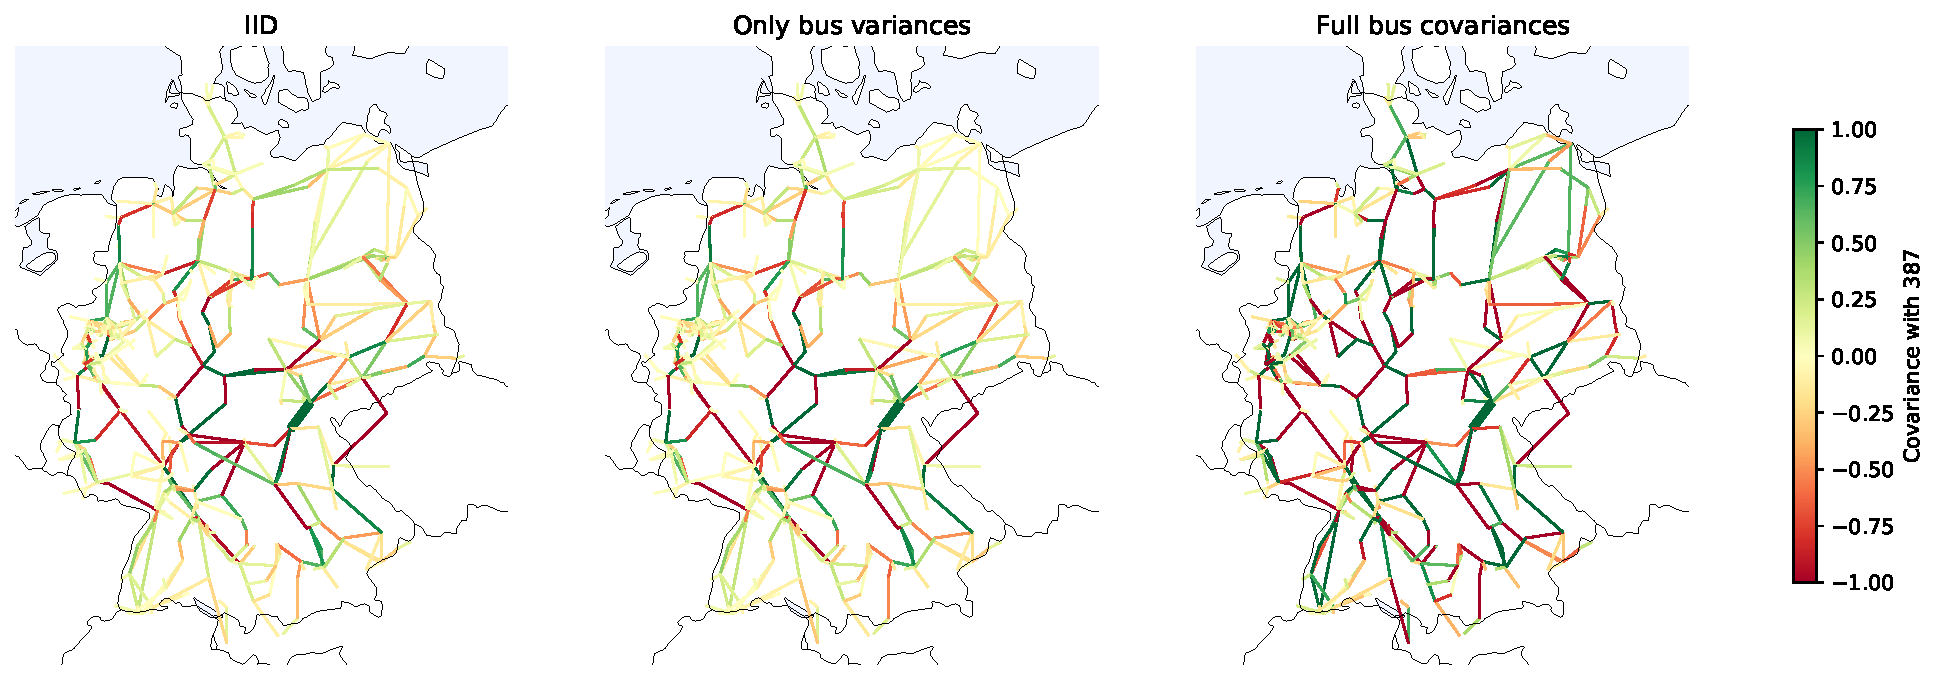
\includegraphics[width=\textwidth]{img/flow_correlation_387_iid_and_justvar_and_fullcov.pdf}
    \caption{}\label{fig:linecov1}
\end{subfigure}
\begin{subfigure}{\textwidth}
    \centering
    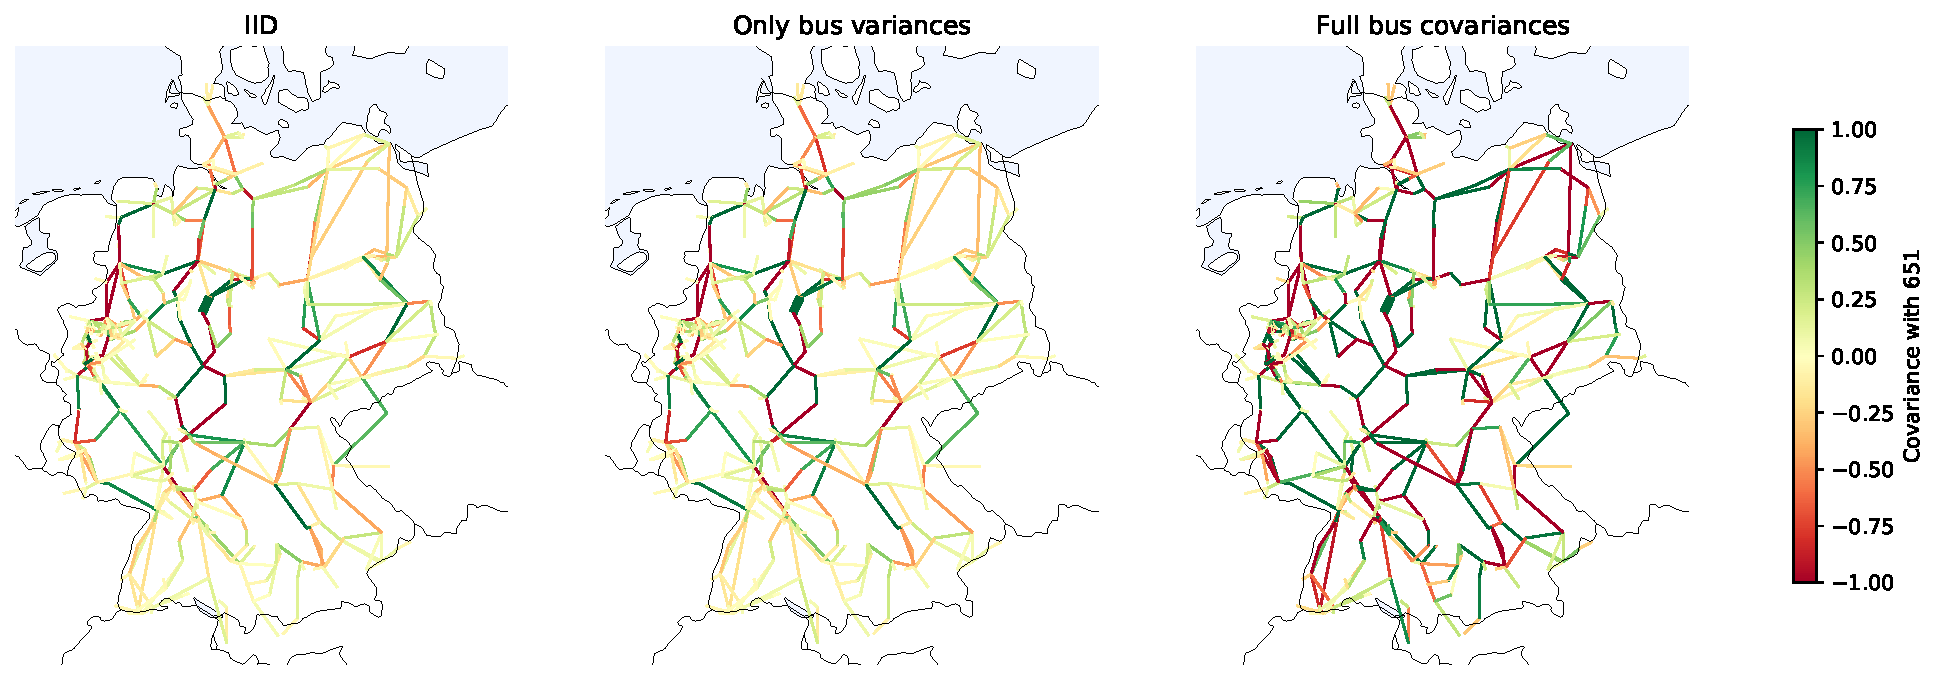
\includegraphics[width=\textwidth]{img/flow_correlation_651_iid_and_justvar_and_fullcov.pdf}
    \caption{}\label{fig:linecov2}
\end{subfigure}
    \caption{Covariance of all lines, relative to the enlarged line. Normalised using installed renewable capacity. Signs (red or green) can be chosen arbitrarily. Absolute covariance is therefore proportional to color \emph{saturation}.}
\end{figure}

The covariance of a random pair of lines is relatively high, when their physical separation (measured either in kilometres or in graph distance) is low. Because weather is correlated, even at high distance, using the bus full covariance might result in higher covariances between lines with high separation. (This was concluded by \cite{Nesti2018emergentfailures}.) 

Using a different bus covariance matrix will likely result in a overall increase or decrease of line covariances. Note, however, that the line covariance matrix is scaled by an arbitrary factor $\epsilon$, so any overall change in covariance has no significance in the model. 

This makes it difficult to compare the three bus covariance matrices, as any absolute difference in line covariance should be ignored. Instead, we will examine the covariance of two lines, \emph{relative to their own variances}. This way, the effect of any absolute, proportional increase in covariance is avoided. First, let us choose a number of lines, and examine the covariances of all other lines with the chosen line, relative to its variance. 

In particular, we are interested in the decay of covariance over distance. \cite{Jung2016} studied the decay of the Line Addition Distribution Factor (difference in flow after adding a line) over distance, also using the SciGRID network. This is not the same as covariance, of course, but both are measures of the \emph{global effect} of local changes in flow. They first determined the largest 2-connected component of the network, and removed all other lines from the model. In the remaining network, they studied the 880 possible additions of short new lines, and found a general \emph{exponential} decay of change in currents as a function of graph distance.

To study the decay of covariance, we collect the geographical separation and covariance (resulting from the three possible bus covariance matrices) of $10^5$ random pairs of lines in the network. Because of power flow physics, these covariances are highly spread out. However, when averaging the covariances in groups of $25 \, \si{\kilo\metre}$ (Figure~\ref{fig:linecovdecay}), we find are able to see the differences in decay. 

\begin{figure}
\centering
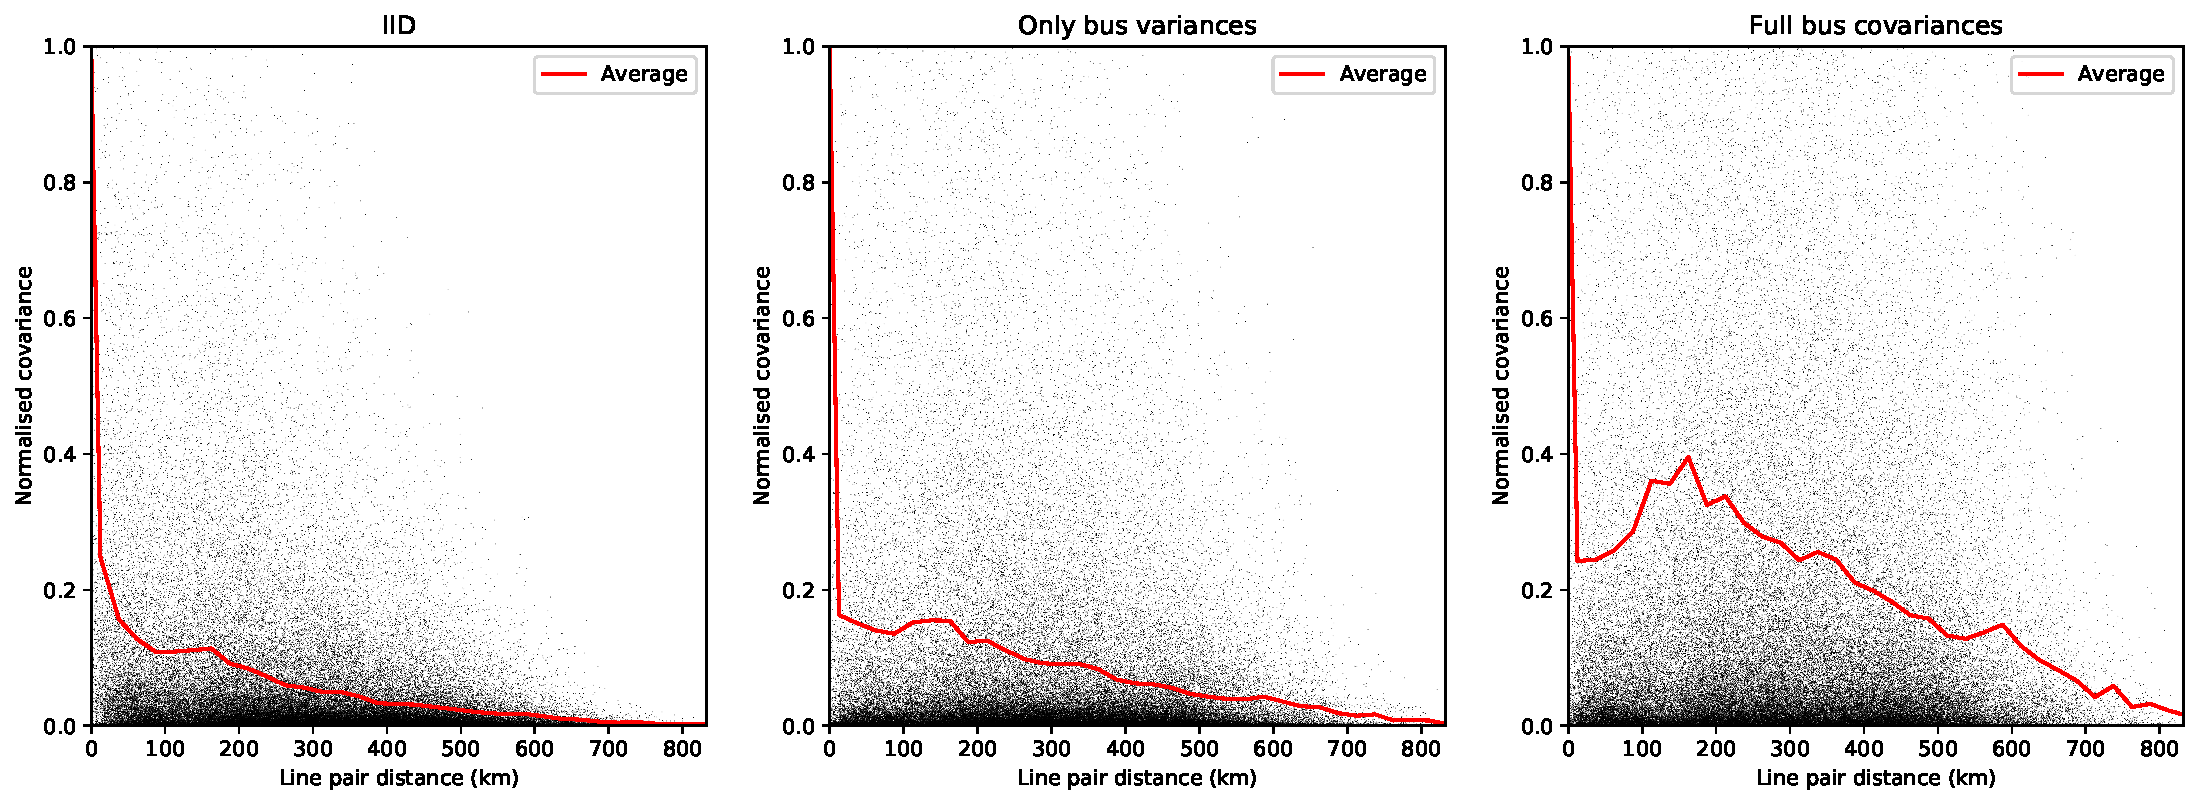
\includegraphics[width=\textwidth]{img/covariance_linepairs_with_average.pdf}
\caption{\label{fig:linecovdecay} For $10^5$ random pairs of lines, the covariance and distance (between line centres) is shown, for three possible bus covariance matrices. The averages (over $25 \, \si{\kilo\metre}$) show that correlated buses increase long-range correlations in line flows. Covariances are normalised using average line variance.}
\end{figure}

 \todo{Maar als je normaliseert op variantie?}
Outage
\towrite{Compare three bus covariance }


\begin{figure}
    \centering
    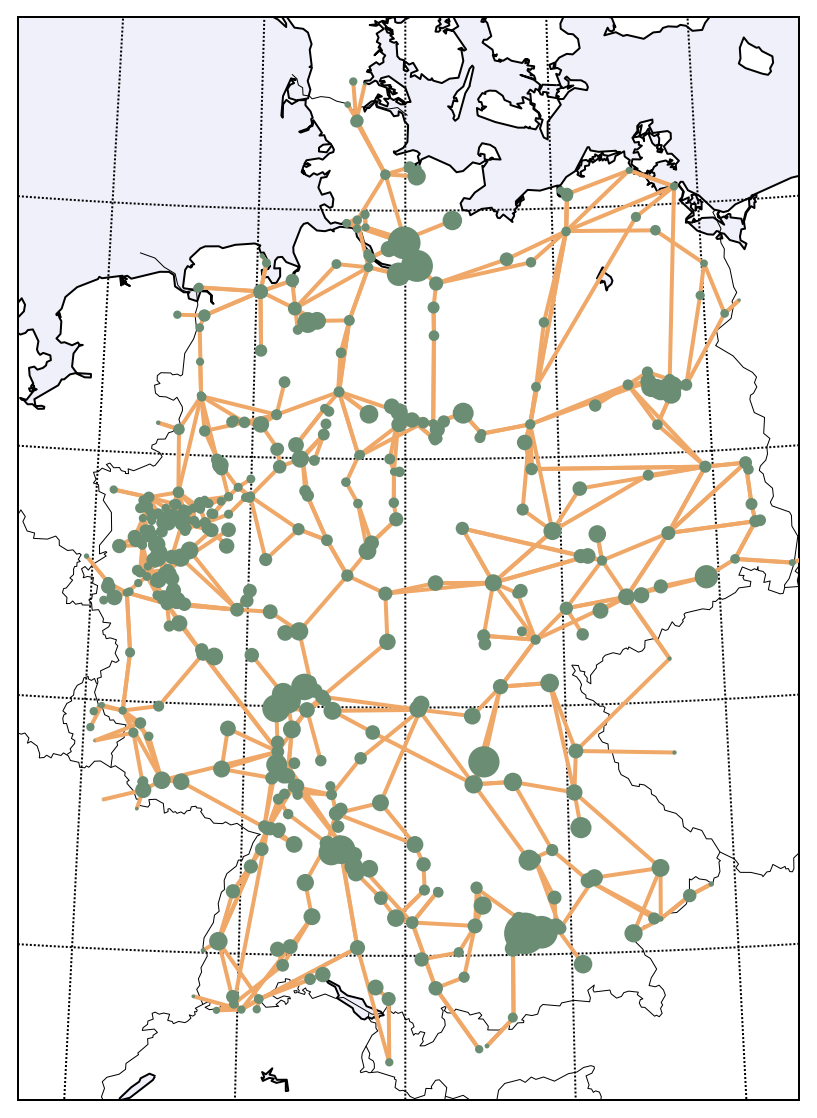
\includegraphics[width=.4\textwidth]{img/load.png}
    \caption{PLACEHOLDER: The load distribution of Germany at ???.}
    \label{fig:loaddistribution}
\end{figure}

\begin{figure}
    \centering
    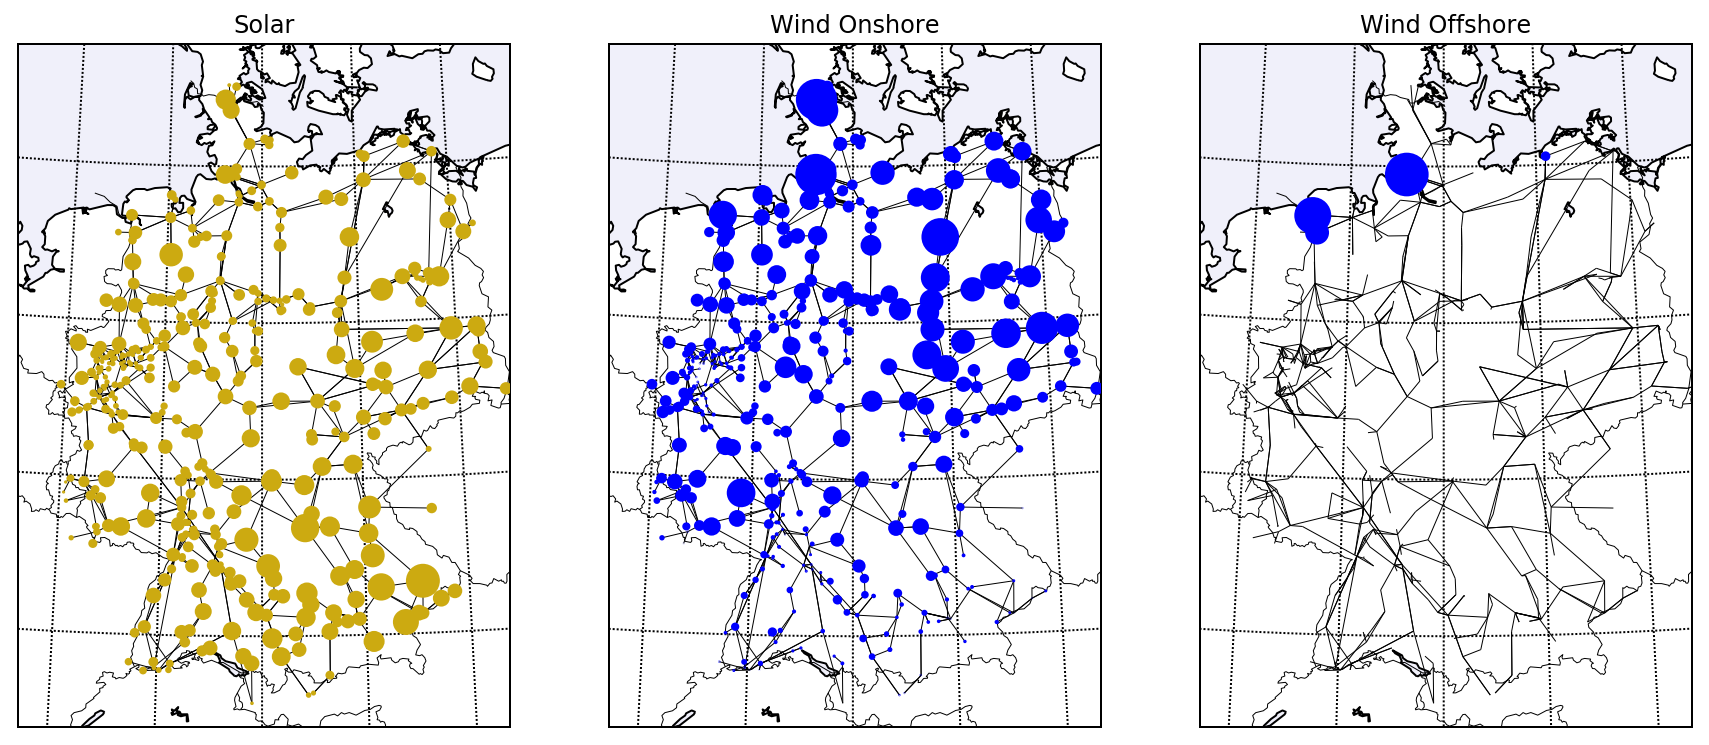
\includegraphics[width=\textwidth]{img/solarwind.png}
    \caption{PLACEHOLDER: Solar, wind onshore, wind offshore generation at ?? in Germany.}
    \label{fig:solarwind}
\end{figure}

\begin{figure}
    \centering
    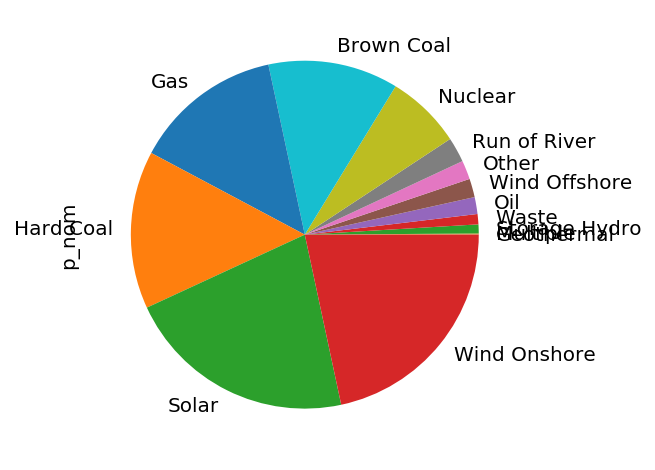
\includegraphics[width=.4\textwidth]{img/genprop.png}
    \caption{PLACEHOLDER: Generation capacity technology shares in Germany in 2011.}
    \label{fig:generationtech}
\end{figure}

\todo{Plotjes van kansen zoals in \label{stochasticpowerinjections}}


\section{Most vulnerable lines}
Using the nominal injection at 1 January, 11:00, we compute the failure probability of each line. The 20 most vulnerable lines are given in Table~\ref{tab:top20}. We identify the same vulnerable lines as \cite{Nesti2018supplemental}, but the ranking is different. This can be attributed to two differences in approach. First, we have combined parallel lines,\footnote{all 20 most vulnerable lines were not part of a parallel combination} which changes the vulnerability order significantly. It is unclear why this changes the result. For comparison, the ranking that we get \emph{without} combining parallels is given in Table~\ref{tab:top20old}, which is more similar that of \cite{Nesti2018supplemental}. The second major difference is the use of a different covariance matrix, although it is reassuring to see that the same lines are identified.\todo{Check hun cov}

\subsection{Cascades}
In addition to the failure probability, we compute the most likely injection to cause that failure, and simulate the resulting cascade. The number of lines that either failed jointly with the initial failure, or failed during the subsequent cascade, is also given in the Table. This extends the result of \cite{Nesti2018supplemental}, which only provides the failure probability.

\towrite{We find that among the 20 most vulnerable lines (at 11:00),

geef percentage dat oke blijft}

\subsubsection{Using the most likely injection}
\towrite{hoe zijn de resultaten anders wanneer we niet de mli nemen?}


\subsection{Evolution of line vulnerabilities}
Of course, the method above can be applied to any nominal injection, not just the injection at 1 January, 11:00. By applying the method to every hour of the first day, we find 24 different rankings, one of which is given in Table~\ref{tab:top20}. This allows us to not only identify lines that are vulnerable at a given point in time, but to find lines that are a \emph{consistent vulnerability}, based on the general use of the transmission network.

Instead of providing 23 additional tables, we have summarised the results of a full day in Figure~\ref{fig:evolution_vulnerabilities}. Here, we see that some lines (like 337) are only vulnerable at one point during the day, while others (298 and 54) have a consistently high overload probability. There is a clear distinction between daytime and night-time, since the time of day determines which covariance matrix is used in the calculation. In fact, this highlights how a change in covariance influences results: some lines are only vulnerable because of the covariances brought upon by solar generation, while others are relatively unaffected.

A most striking result is that the overload probabilities of 25 and 298 are perfectly \emph{constant} for sustained periods, and both are likely to cause a cascade, resulting in an average of 108 and 76 failures, respectively. When examining these two lines in more detail, we find that both are \emph{branches out of the network towards coastal cities of the North Sea}, with high-capacity offshore wind generation. These generators were operating at full capacity during the studied day,\footnote{That is, according to our dataset.} which would cause a constant\footnote{except for the local energy usage, which is relatively small} power injection. Because the lines are \emph{branches} out of the larger graph, the flow through the line is exactly equal to the power injection at its end.

Regarding the subsequent cascades of these two lines, it seems like our model falls short of giving an accurate redistribution of flow, due to the singularity caused by their removal. (No flow redistribution exists that would not change the injection.) 

\begin{figure}[ht]
\begin{subfigure}{\textwidth}
    \centering
    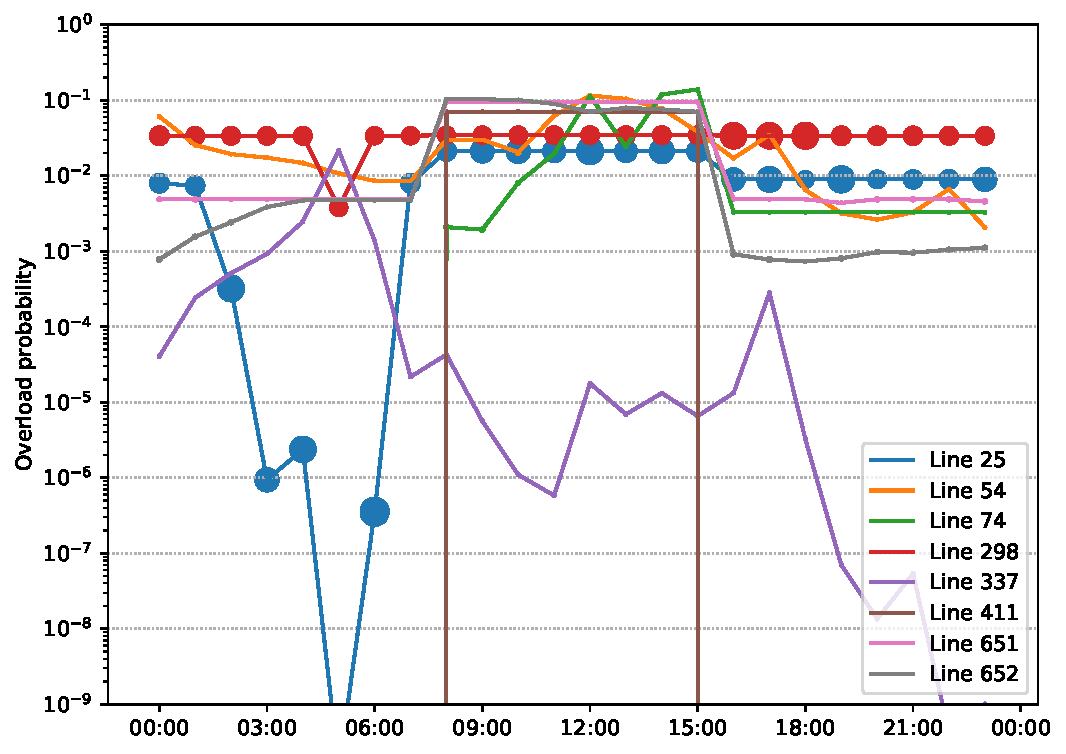
\includegraphics[width=\textwidth]{img/evolution_overload_probs_3.pdf}
    \caption{All lines that are, at any time during the day, among the 3 most vulnerable lines.}\label{fig:evolution_vulnerabilities_3}
\end{subfigure}
\begin{subfigure}{\textwidth}
    \centering
    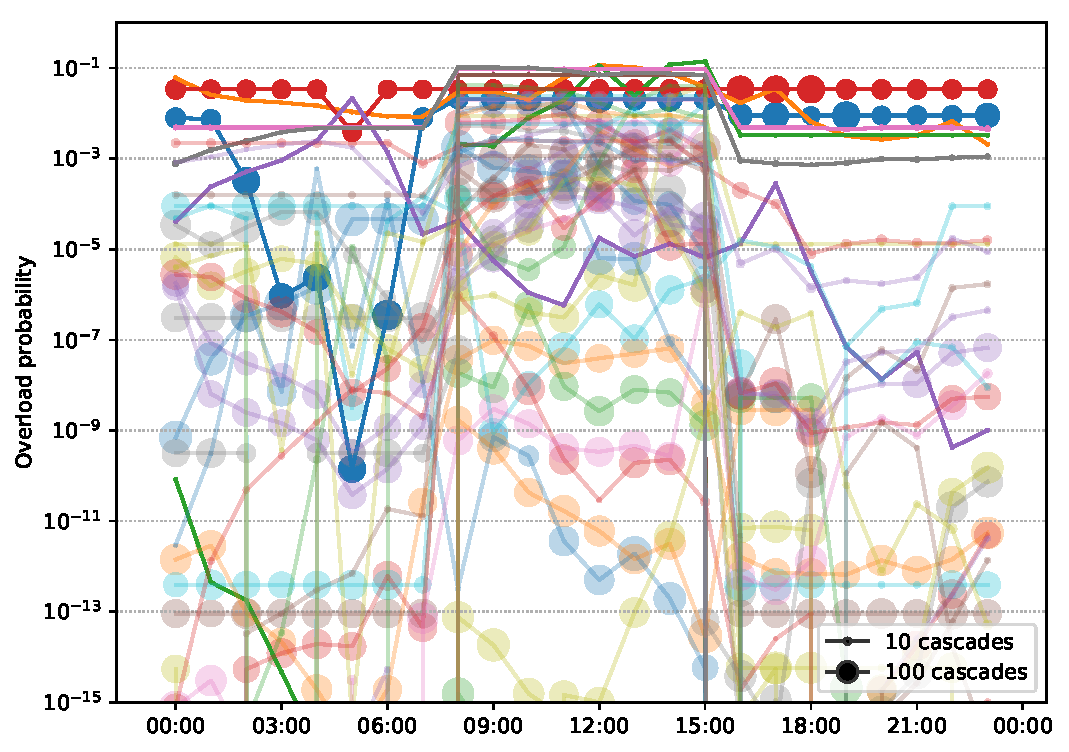
\includegraphics[width=\textwidth]{img/evolution_overload_probs_3_20.pdf}
    \caption{All lines that are, at any time during the day, among the 20 most vulnerable lines.}\label{fig:evolution_vulnerabilities_3_20}
\end{subfigure}
    \caption{\label{fig:evolution_vulnerabilities}Evolution of absolute failure probabilities during 1 January 2011. Dot sizes represent final number of lost lines after the most probable cascade.}
\end{figure}

\begin{figure}[ht]
    \centering
    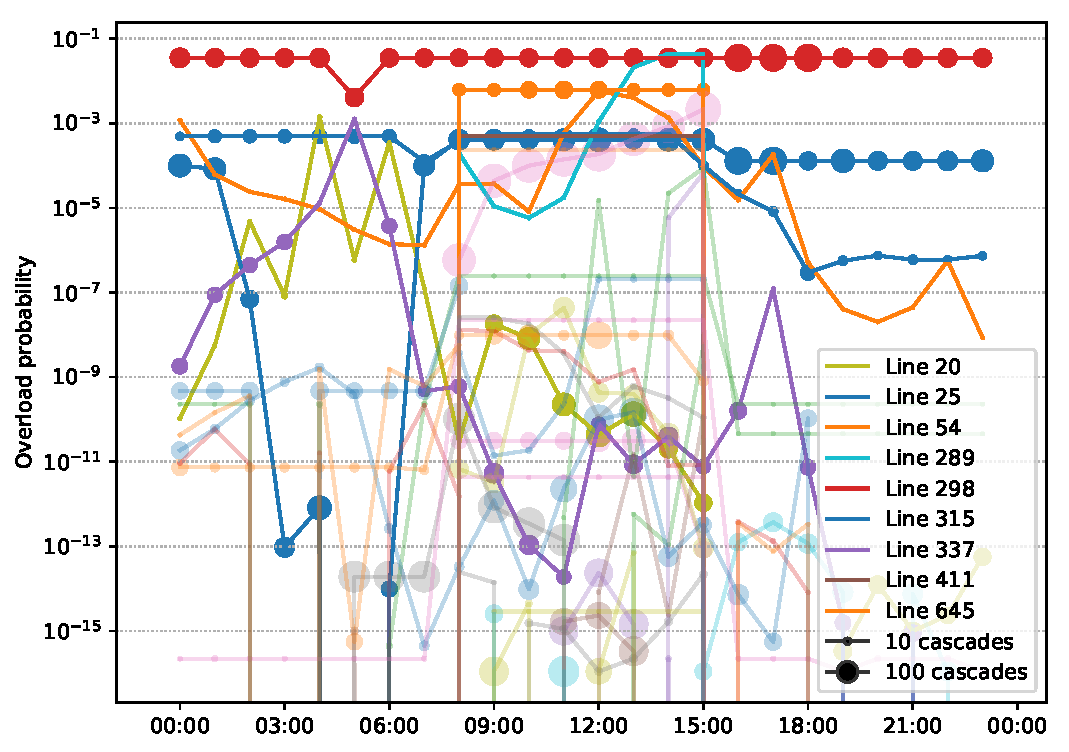
\includegraphics[width=\textwidth]{img/evolution_overload_probs_3_20_IID.pdf}
    \caption{The same as Figure~\ref{fig:evolution_vulnerabilities_3_20}, computed using \emph{uncorrelated} injections.}\label{fig:evolution_vulnerabilities_3_20_IID}
\end{figure}


\section{Lines vulnerable to cascades}
\towrite{}


\begin{table}
\begin{tabular}{lll}
\toprule
$l$ & $\PROB \left[ |\mel{f}_l| \geq 1 \right]$ & $\mel{I}_l$ \\
\midrule
361 & 3.45\hphantom{0}\% &  1.65 \\
516 & 2.91\hphantom{0}\% &  1.79 \\
586 & 2.75\hphantom{0}\% &  1.84 \\
587 & 2.73\hphantom{0}\% &  1.85 \\
803 & 2.02\hphantom{0}\% &  2.10 \\
670 & 1.21\hphantom{0}\% &  2.54 \\
19  & 1.13\hphantom{0}\% &  2.60 \\
302 & 1.08\hphantom{0}\% &  2.64 \\
48  & 1.03\hphantom{0}\% &  2.68 \\
554 & 0.974\% &  2.73 \\
\midrule
488 & 0.971\% &  2.73 \\
809 & 0.824\% &  2.88 \\
28  & 0.748\% &  2.96 \\
810 & 0.728\% &  2.98 \\
29  & 0.396\% &  3.53 \\
27  & 0.355\% &  3.62 \\
389 & 0.247\% &  3.95 \\
390 & 0.245\% &  3.96 \\
486 & 0.235\% &  4.00 \\
249 & 0.056\% &  5.30 \\
\bottomrule
\end{tabular}

\caption{TODO}
\label{tab:top20old}
\end{table}

\section{Previous work}
This thesis was inspired by \cite{Nesti2018emergentfailures}, and we have verified their results. Our results are in overall agreement, with some minor differences. \todo{minder beknopt}

Verschillen:

- lijnen samengevoegd

- geen arma maar diff

- cascades gegeven van top 10


Kritiek op nesti:

- ARMA modellen, logisch? nodig? goede modellen?

- geeft cascades niet van top 10

- ze nemen een contingency factor van 0.7 bij de OPF (arbitrair) maar voor de analyse van cascades niet. (toch?)




\clearpage
\end{document}